\documentclass[12pt]{beamer}
\usepackage{graphicx}
\graphicspath{{./images/}}
\usepackage{float}
\usetheme{Warsaw}
\author{Anubhav Mehra}
\title{Digital Image Processing}
\institute{S.S.J. Campus, Almora}
\date{\today}


\begin{document}
\maketitle
\begin{frame}{Introduction}
 \textbf{What is Digital Image Processing?} \\
      \begin{itemize}
      \item {
        Digital Image \\
          — a two-dimensional function \\
              x and y are spatial coordinates \\
              The amplitude of f  is called intensity or gray level at the point (x, y) \\
              Components are called pixels.
      }
      \item {
       Digital Image Processing \\ 
          — process digital images by means of computer\\ [0.5ex]
         low-level: inputs and outputs are images \\ 
         mid-level: outputs are attributes extracted from input images \\
         high-level: an ensemble of recognition of individual objects \\
      }
      \end{itemize}


\end{frame}
\begin{frame}{Components}
\begin{figure}[H]
\begin{center}
\caption{Components of Image Processing}
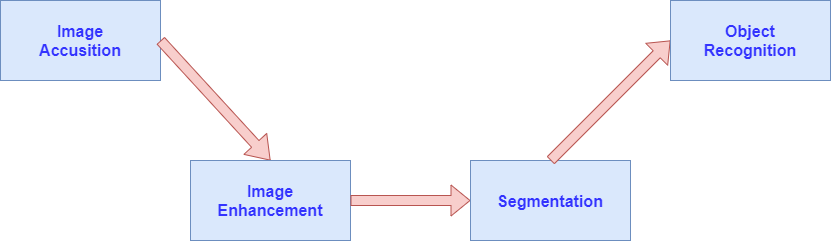
\includegraphics[scale=0.3]{com.png}
\end{center}
\end{figure}
\end{frame}

\begin{frame}{ Process of Image Acquisition}
The Image Acquisition is purely Hardware
Dependent Process, in which reflected light energy
from the object being imaged is converted into
electrons and spread over the internal sensor chip
which is like a 2-D array of cells is cell is called
photosite and contain amount of charges which is
further converted to digital form using Analog to
Digital Converter. \\[1ex]

Now this digital image can be used for
enhancement, restoration, segmentation and other
manipulations
\end{frame}

\begin{frame}{Image Acquisition}
\begin{figure}[H]
\begin{center}
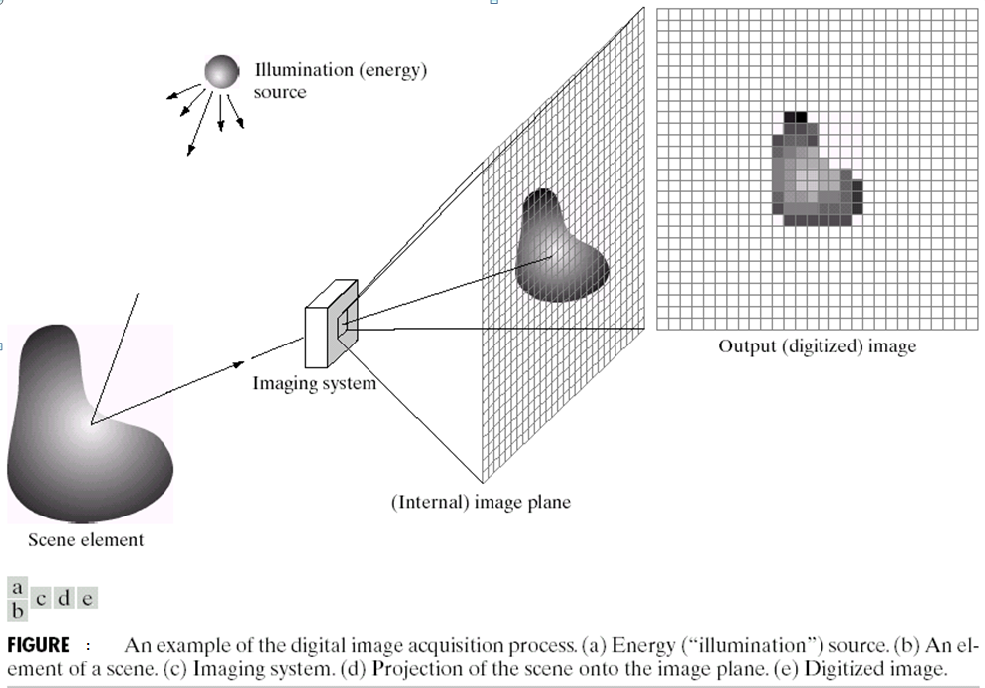
\includegraphics[scale=0.4]{acq.png}
\end{center}
\end{figure}
\end{frame}


\begin{frame}{Image Enhancement}
\begin{itemize}
\item \textbf{Image Enhancement process} consists of collection of techniques that seek to improve the visual appearance of the image or to convert the image to a form better suited for analysis.

\item \textbf{The principle idea} of image enhancement is to modify the attributes of an image to make it more suitable for 

\begin{figure}[H]
\begin{center}
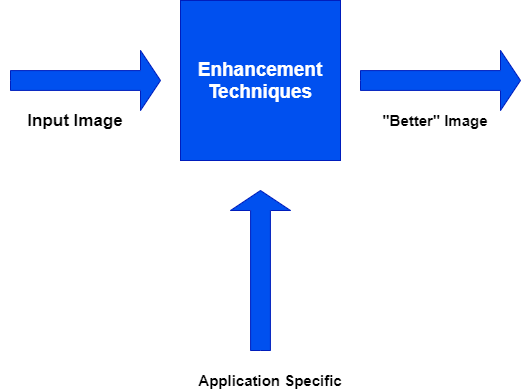
\includegraphics[scale=0.3]{enh.png}
\end{center}
\end{figure}
\end{itemize}
\end{frame}

\begin{frame}{Enhancement Techniques}
\large The image enhancement techniques can be divide into two main categories:
\normalsize
\only<1>{
\begin{itemize}
\item Spatial Domain Techniques \\
These techniques are performed to the image plane itself and they are based on direct manipulation of pixels in an image. \\
The operation can be formulated as $g(x,y) = T[f(x,y)]$, where $g$ is the output, $f$ is the input and $T$ is some operation on $f$   defined over some neighborhood of $(x,y)$. \\
e.g., \textbf{Contrast Enhancement, Sharpening.}
\end{itemize}
}
\only<2> {
\begin{itemize}
\item<2> Frequency Domain Techniques \\
In this techniques the image is first transferred into frequency domain using Fourier Transform. Then the Enhancement operations are performed on Fourier transform of the image and then the Inverse Fourier Transform is calculated to get the resultant image.

$f(x,y) \rightarrow F(u,v) rightarrow G(u,v) = H(u,v)F(u,v), G(u,v) \rightarrow g(x,y) $ \\
e.g. \textbf{Low-pass, High-pass filtering.}
\end{itemize}
}
\end{frame}
\begin{frame}{Segmentation}
\textbf{Image Segmentation}
 is the process of partitioning a digital image into multiple segments (sets of pixels, also known as image objects). The goal of segmentation is to simplify and/or change the representation of an image into something that is more meaningful and easier to analyze. Image segmentation is typically used to locate objects and boundaries (lines, curves, etc.) in images. 
 \begin{figure}[H]
 \begin{center}
 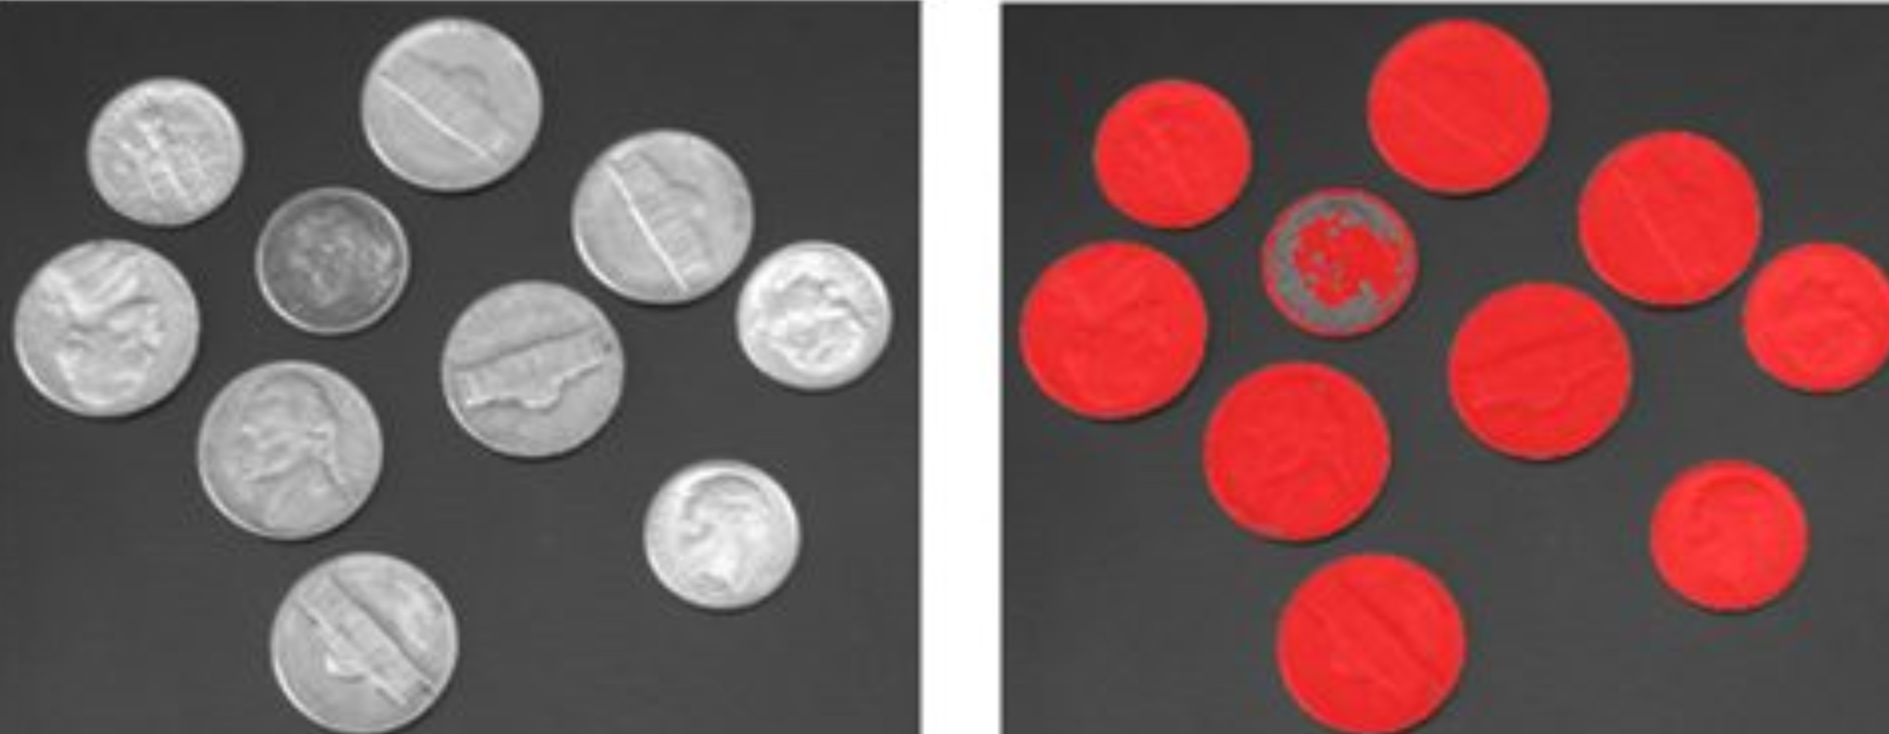
\includegraphics[scale=0.2]{coins.png}
 \end{center}
 \end{figure}
\end{frame}

\begin{frame}{Segmentation Techniques}
There are various segmentation techniques. Some are mentioned below:
\begin{itemize}
\item Histogram Based \\
\begin{enumerate}
\item Thresholding
\item Clustering
\end{enumerate}
\item Motion Based
\item Discontinuity Based \\
\begin{enumerate}
\item Point detection
\item Line detection
\item Edge detection
\end{enumerate}
\item Similarity Based \\
\begin{enumerate}
\item Region growing
\end{enumerate}
\end{itemize}
\end{frame}
\begin{frame}{Object Recognition}
\textbf{Object recognition} is a general term to describe a collection of related computer vision tasks that involve identifying objects in digital photographs.
\\ [1ex]
These tasks often comprises of the following tasks:-
\\[1ex]
\begin{figure}
\begin{center}
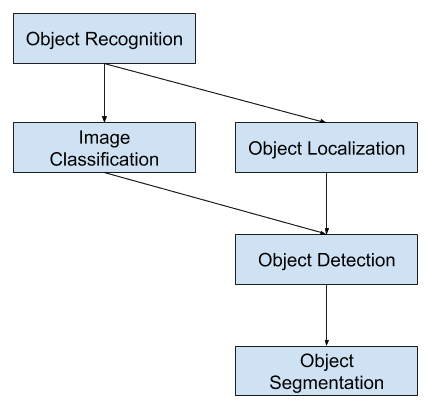
\includegraphics[scale=0.4]{obj.png}
\end{center}
\end{figure}
\end{frame}
\begin{frame}{Object Recognition Tasks}
\small
We can distinguish between these three computer vision tasks:
\begin{itemize}

\item \textbf{Image Classification:} Predict the type or class of an object in an image.
\begin{itemize}
\tiny
\item \textbf{Input:} An image with a single object, such as a photograph.
\item Output: A class label (e.g. one or more integers that are mapped to class labels).
\end{itemize}
\item \textbf{Object Localization:} Locate the presence of objects in an image and indicate their location with a bounding box.
\begin{itemize}
\tiny
\item \textbf{Input:} An image with one or more objects, such as a photograph.
\item \textbf{Output:} One or more bounding boxes (e.g. defined by a point, width, and height).
\end{itemize}
\item \textbf{Object Detection:} Locate the presence of objects with a bounding box and types or classes of the located objects in an image.
\begin{itemize}
\tiny
\item \textbf{Input:} An image with one or more objects, such as a photograph.
\item \textbf{Output:} One or more bounding boxes (e.g. defined by a point, width, and height), and a class label for each bounding box.
\end{itemize}
\end{itemize}
\end{frame}
\begin{frame}{Question and Answers}
\begin{figure}
\begin{center}

\includegraphics[scale=0.2]{thank.jpg}
\end{center}
\end{figure}
\tiny
The slides for the today's presentation can be downloaded from: \\

https://github.com/AnubhavMehraCS/Paper2/raw/main/imageprocessing.pdf \\ [1ex]
\small
\textbf{References}:
\tiny
\begin{enumerate}
\item https://www.slideshare.net/OECLIBOdishaElectron/image-processing-ppt-79369981
\item https://www.slideshare.net/surabhiks5/image-enhancement-ppt-nal2
\item https://en.wikipedia.org/wiki/Image\_segmentation
\item https://machinelearningmastery.com/object-recognition-with-deep-learning/
\end{enumerate}
\normalsize
\end{frame}
\end{document}